\chapter{Implementation}\label{sec3}
This chapter examines the implemented solution %to achieve the 
that aims to produce a modular quantum machine learning tool. The components of this solution are separated into subsections within which the important functions are explained. These subdivisions are used with the intent to provide a further understanding of the logic used in the system, thus providing an in-depth understanding into the overall structure.


\section{Data Encoding}
With the knowledge gained about quantum gates and operations from Chapter \ref{BackgroundLit} we can now observe them in use. However, the question of how to use classical data with a quantum circuit arises. There are a number of data encoding techniques available and this section explores \emph{amplitude encoding} and \emph{feature mapping}.

\subsection{Amplitude Encoding}
Amplitude encoding is a technique to encode classical information into amplitude of quantum states. It maps the coordinates of a vector into the values of the amplitudes of a quantum state. %This is carried out by preparing the data through normalisation and feature padding and the datapoint angles are then extracted from this prepared data. The angle are rotated to encoded them within the Bloch sphere. this encoding allows for the data to be encoded into a quantum states. 
As explained in Section \ref{AmpEnBack}, this type of data encoding is very useful for smaller datasets with multiple features; however, it could increase resource requirements \citep{QiskitFMap}.  


\vspace{0.3cm}
\textbf{\underline{Data Preparation}}
\label{PrepData}

Amplitude encoding requires the mapped data vector to be normalised and to have a power-of-two dimension. To achieve this, data preparation through the use of data normalisation and data padding is needed.

Taking the desired dataset, the required variables are chosen, padded if necessary and the data is then re-normalised. For example, the Iris dataset is composed of four variables labelled -1 or 1. Keeping the features in the two first columns, the features can be transformed using the labels 0 and 1. This data is then padded with constant values and re-normalised to result in a unitary vector.

%%%%%%%%%%%%%%%%%%%%%%%%%%%%%%%%%%%%%%%%
\begin{figure}[H]
      \centering
      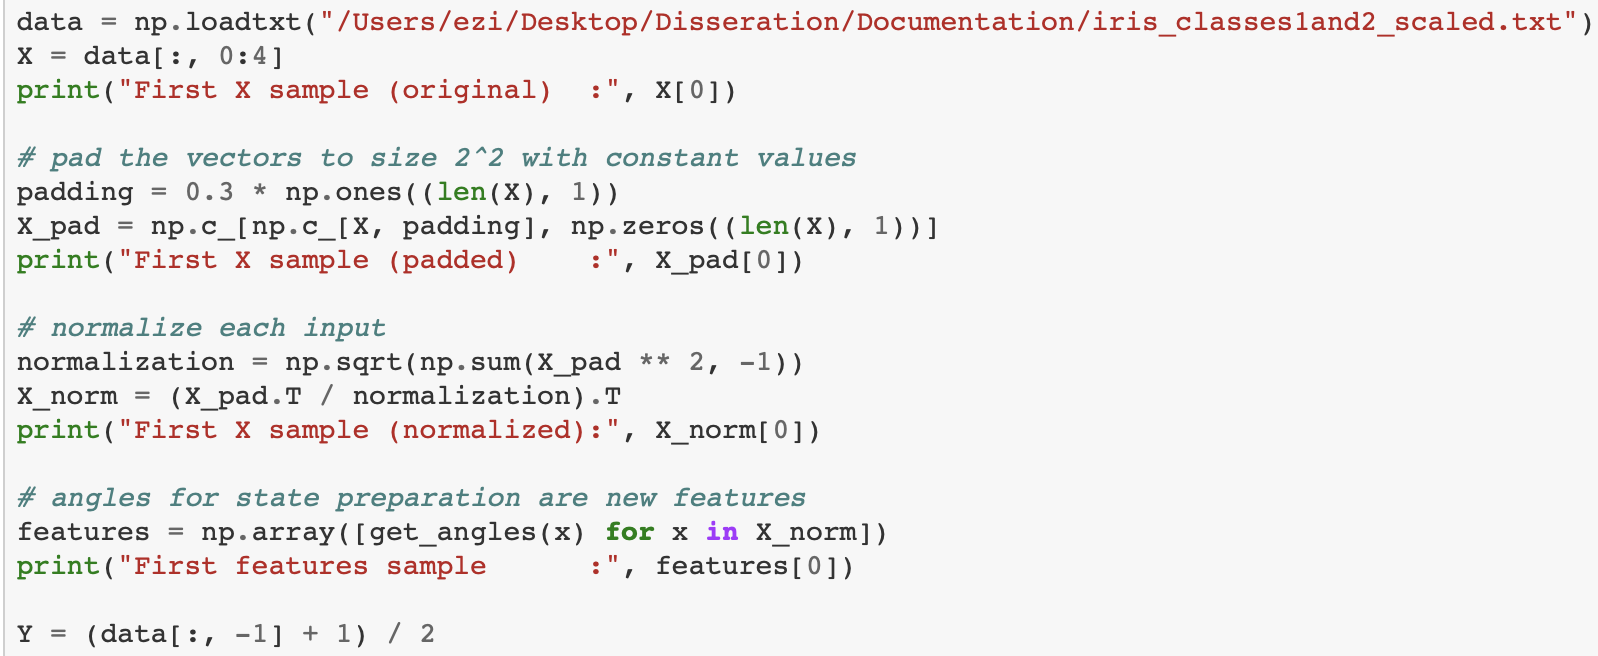
\includegraphics[scale=0.56]{background/AmpDataPrep.png}
      \caption{Amplitude Encoding: Data Preparation }
      \label{AMPDataPrep}
\end{figure}
%%%%%%%%%%%%%%%%%%%%%%%%%%%%%%%%%%%%%%%%


\vspace{0.3cm}
\textbf{\underline{Data Mapping }}

To encode the prepared data into a quantum state, the data must be rotated in the Bloch sphere. The amplitude circuit makes use of the Ry gate to rotate single qubits through an angle around the $y-axis$. Given that the unitary vector has four dimensions, five angles with the function \texttt{get$_-$angles()} shown in Figure \ref{AMPAng} can be extracted; these angles then serve as arguments to encode the quantum circuit.

%%%%%%%%%%%%%%%%%%%%%%%%%%%%%%%%%%%%%%%%
\begin{figure}[H]
      \centering
      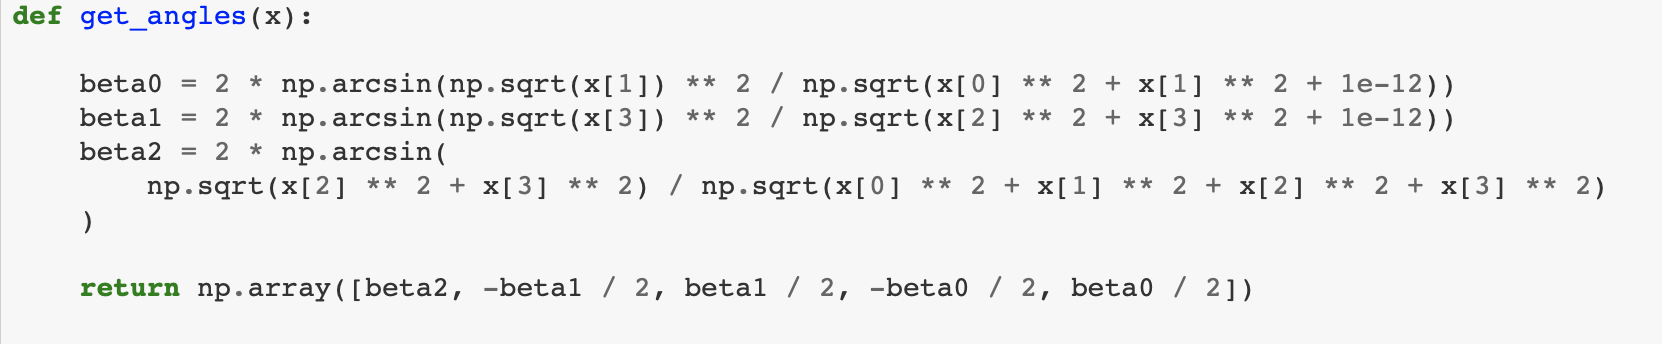
\includegraphics[scale=0.56]{background/GetAngles.png}
      \caption{Getting the Angles Code }
      \label{AMPAng}
\end{figure}
%%%%%%%%%%%%%%%%%%%%%%%%%%%%%%%%%%%%%%%%


%%%%%%%%%%%%%%%%%%%%%%%%%%%%%%%%%%%%%%%%
\begin{figure}[h]
      \centering
      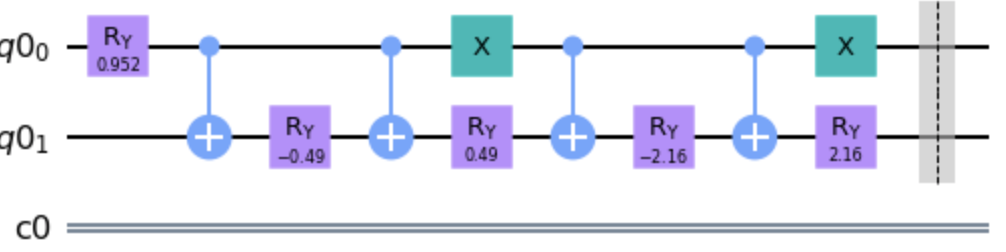
\includegraphics[scale=0.7]{background/RYGate.png}
      \caption{Amplitude Encoding: Circuit }
      \label{AMPCiruit}
\end{figure}
%%%%%%%%%%%%%%%%%%%%%%%%%%%%%%%%%%%%%%%%


\subsection{Feature Mapping}
\label{FMapp}
Feature mapping reduces the amount the resources required to describe a large set of data.
As described in Section \ref{FMapBack}, unlike amplitude encoding, the data points are converted into vectors using the V($\phi(\overrightarrow{x_i})$ function as quantum data is represented as vectors; this vector data can more easily encoded into a quantum space. 

\vspace{0.3cm}
\textbf{\underline{Data Preparation}}

Taking the Iris data set as our example in Figure \ref{DPrep}, the number of datapoints one wishes to test  needs to be specified. Similar to amplitude encoding, the desired data first needs to be normalised before it can be mapped. 

%%%%%%%%%%%%%%%%%%%%%%%%%%%%%%%%%%%%%%%%
\begin{figure}[H]
      \centering
      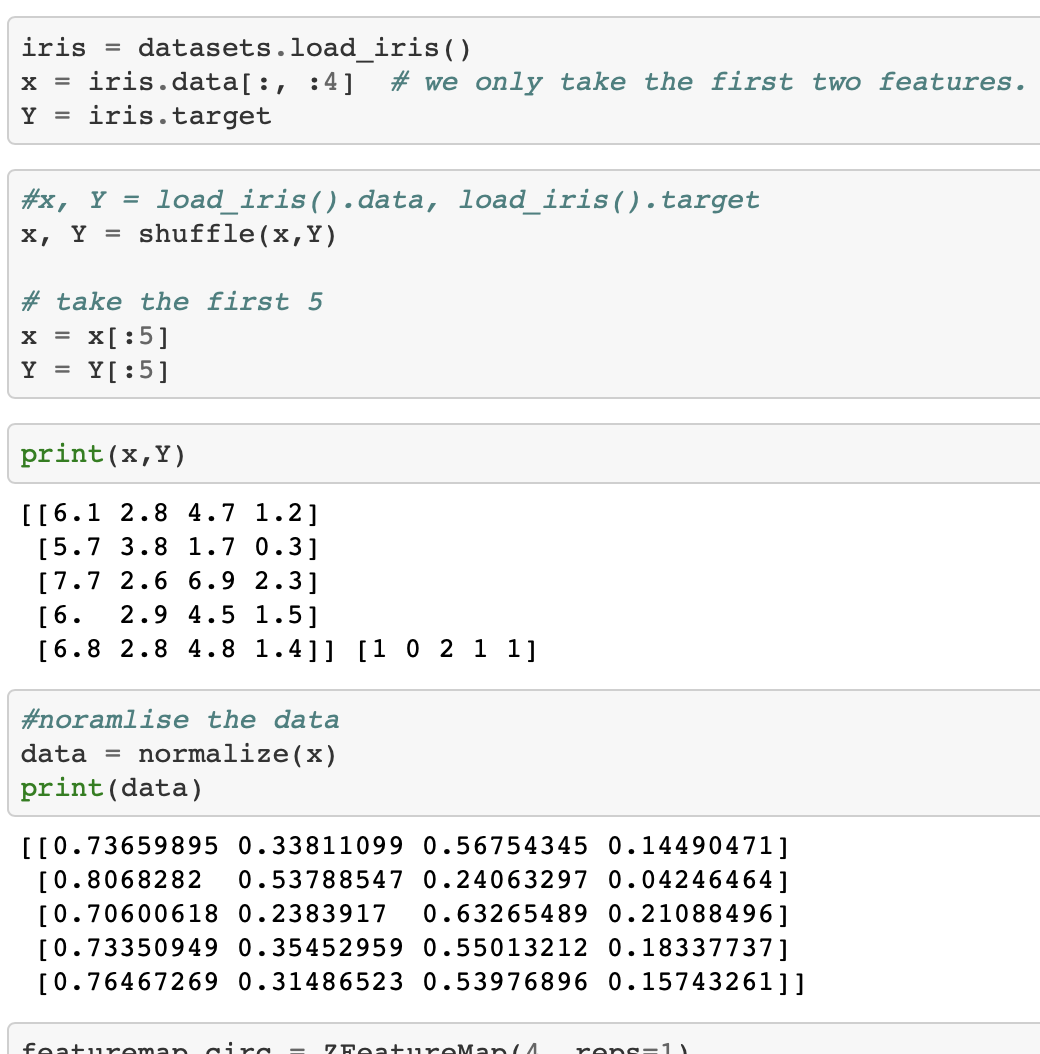
\includegraphics[scale=0.5]{background/DataNorm.png}
      \caption{Data Preparation}
      \label{DPrep}
\end{figure}
%%%%%%%%%%%%%%%%%%%%%%%%%%%%%%%%%%%%%%%%

\vspace{0.6cm}
\textbf{\underline{Data Mapping}}\label{FMapIMPle}

There are different types of feature maps available: 
\begin{enumerate}
 
\item \texttt{PauliFeatureMap}: The PauliFeatureMap is the general form and it allows for the creation of feature maps using different gates.

\item \texttt{ZFeatureMap}: The ZFeatureMap is the first-order evolution of the PauliFeatureMap.% circuit.

\item \texttt{ZZFeatureMap}: The ZZFeatureMap is the second-order evolution of the PauliFeatureMap. %circuit.

\end{enumerate}
%\vspace{0.1cm}

The Qiskit built in command, shown in Figure \ref{FMImp},  allows any of these feature maps to be selected. %are initially imported and whichever works best for the user is the one chosen.
%%%%%%%%%%%%%%%%%%%%%%%%%%%%%%%%%%%%%%%%
\begin{figure}[H]
      \centering
      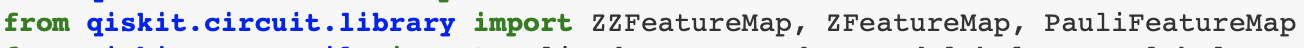
\includegraphics[scale=0.6]{background/FMapImp.png}
      \caption{Feature Map Import Code}
      \label{FMImp}
\end{figure}
%%%%%%%%%%%%%%%%%%%%%%%%%%%%%%%%%%%%%%%%

The feature map is then called as a dataframe, specifying the number of features and the desired number of repetitions. Figure \ref{FMSpec} details an implementation with four features and one repetition. 

%%%%%%%%%%%%%%%%%%%%%%%%%%%%%%%%%%%%%%%%
\begin{figure}[H]
      \centering
      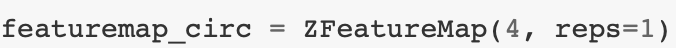
\includegraphics[scale=0.7]{background/FMSpec.png}
      \caption{Specifying the features and repetitions for the Feature Map}
      \label{FMSpec}
\end{figure}
%%%%%%%%%%%%%%%%%%%%%%%%%%%%%%%%%%%%%%%%

The data is then assigned to the circuit parameters, after which the circuit containing the feature map %circuit with 
is combined with the assigned parameters of the second datapoint. 
Using the Qiskit code in Figure \ref{FMFun}, the previous two points can be looped through to ensure the feature mapping is applied to every data point in the dataset. 

%%%%%%%%%%%%%%%%%%%%%%%%%%%%%%%%%%%%%%%%
\begin{figure}[H]
      \centering
      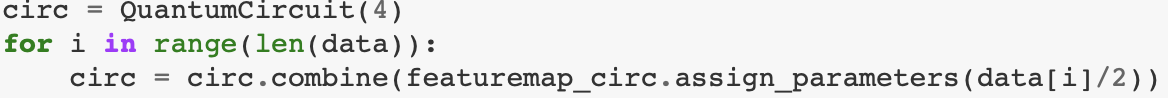
\includegraphics[scale=0.7]{background/FMRun.png}
      \caption{Feature Map Loop Application }
      \label{FMFun}
\end{figure}
%%%%%%%%%%%%%%%%%%%%%%%%%%%%%%%%%%%%%%%%


\subsection{SWAP Gate}

When looking at the QkNN implementation in Section \ref{ImpleQkNN}, the data is stored in qubit one. When encoding the data using feature mapping, the encoded data is in qubits two and three. To reduce the circuit and ensure all data points are encoded into qubit one requires the use of a SWAP Gate.

As illustrated in Figure \ref{SWAPLogic}, SWAP gates allow for the movement of information around in a quantum circuit without the loss of information. The SWAP gate is implemented by calling the Qiskit \texttt{swap} function. %to do so we will call the swap function in Qiskit. 
This function ensures that all data stored in qubit three is now located in qubit two.
This SWAP operation is then repeated with qubit two and qubit one, allowing for the complete transfer of data to qubit one. 

%%%%%%%%%%%%%%%%%%%%%%%%%%%%%%%%%%%%%%%%
\begin{figure}[H]
      \centering
      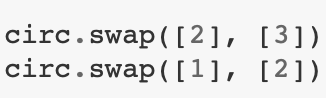
\includegraphics[scale=0.7]{background/SWAPCode.png}
      \caption{SWAP Gate: Code }
      \label{SWCode}
\end{figure}
%%%%%%%%%%%%%%%%%%%%%%%%%%%%%%%%%%%%%%%%

%%%%%%%%%%%%%%%%%%%%%%%%%%%%%%%%%%%%%%%%
\begin{figure}[H]
      \centering
      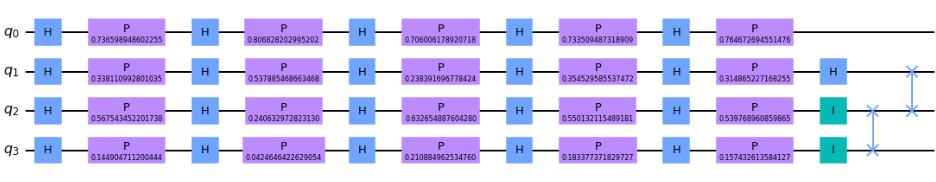
\includegraphics[scale=0.5]{background/SWAPCir.png}
      \caption{SWAP Gate: Circuit Application }
      \label{SWCircuit}
\end{figure}
%%%%%%%%%%%%%%%%%%%%%%%%%%%%%%%%%%%%%%%%
 

\section{Circuit Design}
%With the knowledge gained about quantum gates and operations from Section \ref{BackgroundLit}, we can now observe them in use. 

With the knowledge of how to encode classical data into a quantum state, the newly encoded quantum data can now be used by quantum machine learning algorithms. %  and implement our desired quantum circuit,
 This section explores the implementation of pure quantum and quantum enhanced machine learning algorithms such as: Quantum k-Nearest Neighbour and Quantum Support Vector Mechanism, along with examining a quantum search algorithm, Grover's  Search algorithm.

 The Quantum k-Nearest Neighbour implementation is examined in detail in order to illustrate the use of quantum gates and to further understand their applications. %allowing us to understand how to implement quantum gates in Qiskit. 
  The Quantum Support Vector Mechanism and Grover's Search algorithm are presented in a more shallow sense; however, %different
  two configuration options are provided for each.

\subsection{Quantum k-Nearest Neighbour (QKNN)}\label{ImpleQkNN}

The implemented QkNN algorithm follows the steps laid out in the work \emph{Quantum Algorithm for k-Nearest Neighbours Classification Based on the Metric of Hamming Distance} \citep{wiebe2014quantum}.

%%%%%%%%%%%%%%%%%%%%%%%%%%%%%%%%%%%%%%%%
\begin{figure}[H]
      \centering
      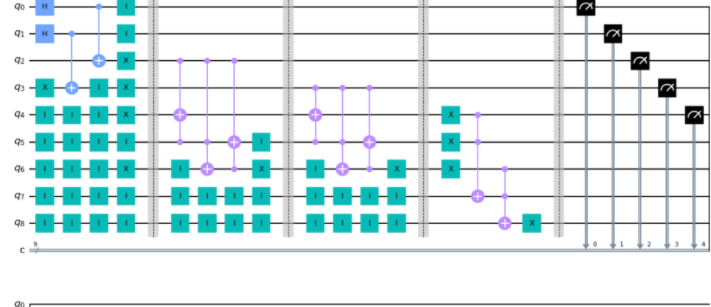
\includegraphics[scale=0.5]{background/FullKNN.png}
      \caption{Completed Quantum K-Nearest Neighbour Circuit}
      \label{FKNN}
\end{figure}
%%%%%%%%%%%%%%%%%%%%%%%%%%%%%%%%%%%%%%%%
This discussion will begin from step two of the main steps from \cite{Kaye}. To provide an overview of the operations, the qubits are first placed into superposition, after which two addition operations are applied to the circuit, followed by an OR operation, as seen in Figure \ref{FKNN}. Each of the sections in this QkNN implementation are explored through the partitioned line brakes shown in Figure \ref{FKNN} %will be explored as partitioned by the line breaks.



\vspace{0.4cm}
\textbf{\underline{Superposition Transformation}}
\vspace{0.1cm}

Figure \ref{QSUP01} is a dissection of Figure \ref{QSUP}, it shows the qubits that have the encoded data (qubit zero and qubit one) being placed into superposition, and they are then entangled with qubit two and qubit three respectively. As discussed in Section \ref{QEC}, this entanglement with other qubits protects \emph{the information stored in qubits by not storing this information in individual qubits but rather in patterns of entanglement among many qubits.} This is a form of Quantum Error Correction, which protects the circuits \emph{quantum information from errors that are primarily due to decoherence and quantum noise}.

%%%%%%%%%%%%%%%%%%%%%%%%%%%%%%%%%%%%%%%%
\begin{figure}[H]
      \centering
      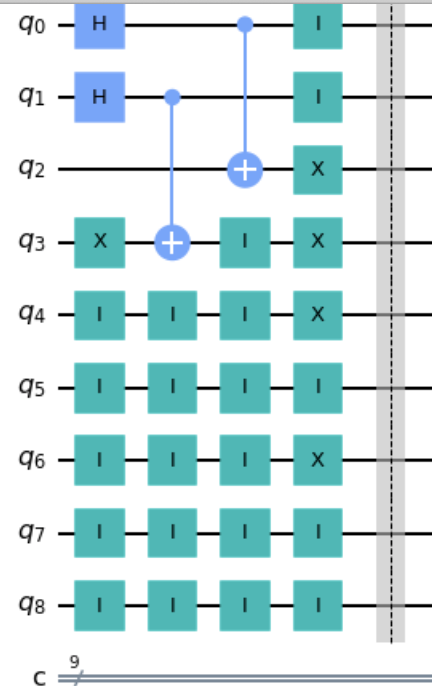
\includegraphics[scale=0.2]{background/SuperPos.png}
      \caption{Quantum K-Nearest Neighbour Circuit: Superposition}
      \label{QSUP}
\end{figure}
%%%%%%%%%%%%%%%%%%%%%%%%%%%%%%%%%%%%%%%%

Figure \ref{QSUP01} displays the unclassified quantum state in qubit zero along with qubit one representing the training set. 
In order to encode both registers into superposition a Hadamard (H) gate is applied. 
%%%%%%%%%%%%%%%%%%%%%%%%%%%%%%%%%%%%%%%%
\begin{figure}[H]
      \centering
      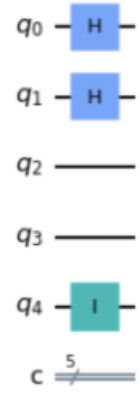
\includegraphics[scale=0.4]{background/sup01.png}
      \caption{Quantum K-Nearest Neighbour Circuit: Superposition qubit zero and one}
      \label{QSUP01}
\end{figure}
%%%%%%%%%%%%%%%%%%%%%%%%%%%%%%%%%%%%%%%%
The states of qubit zero and qubit one are then entangled with qubits two and three, this allows for the superposition states to be mirrored in qubit two and three, respectively. This is implemented using a controlled not operation (CNOT) as demonstrated in Figure \ref{QMir}. In regard to Figure \ref{QMir}, an identity gate is observed on qubit four, this gate ensures no operation is applied to that qubit for one unit gate of time.


%%%%%%%%%%%%%%%%%%%%%%%%%%%%%%%%%%%%%%%%
\begin{figure}[H]
      \centering
      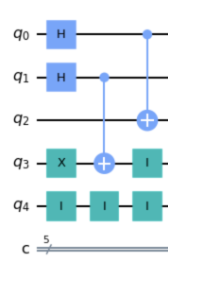
\includegraphics[scale=0.7]{background/Copy23.png}
      \caption{Qubit mirroring: Circuit}
      \label{QMir}
\end{figure}
%%%%%%%%%%%%%%%%%%%%%%%%%%%%%%%%%%%%%%%%


%%%%%%%%%%%%%%%%%%%%%%%%%%%%%%%%%%%%%%%%
\begin{figure}[H]
      \centering
      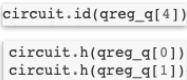
\includegraphics[scale=0.6]{background/SUp1COde.png}
      \caption{Qubit mirroring: Code}
      \label{QSUPCo}
\end{figure}
%%%%%%%%%%%%%%%%%%%%%%%%%%%%%%%%%%%%%%%%




\vspace{0.5cm}
\textbf{\underline{Addition Operations}}
\vspace{0.1cm}


Figure \ref{QAIns} implements an initial A+D addition,
using the entangled data in qubit two and three labelled as D0 and D1 respectively.


Taking qubit four as A0 and qubit five as A1, the following addition is preformed so as to satisfy the complete addition operation:

	\hspace{0.35\textwidth}	A0 + A1 = D0
	
	\hspace{0.35\textwidth}	A0 + A1 = D1
	
%%%%%%%%%%%%%%%%%%%%%%%%%%%%%%%%%%%%%%%%
\begin{figure}[H]
      \centering
      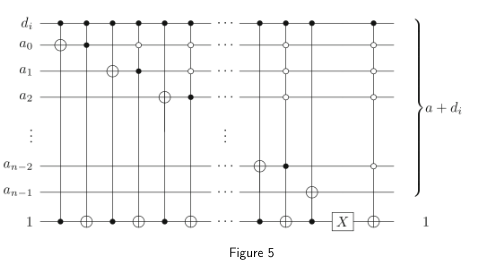
\includegraphics[scale=0.65]{background/AdIns.png}
      \caption{Addition operation illustrated in \citep{Kaye}}
      \label{QAIns}
\end{figure}
%%%%%%%%%%%%%%%%%%%%%%%%%%%%%%%%%%%%%%%%

A toffoli gate is used to carry out these additions, with the first addition operation being implemented following these steps:

\begin{enumerate}
\item Taking qubit two, qubit four is set as the target and qubit five is the control. 
\vspace{0.3cm}

\item Then with qubit two and five as the controls, qubit six is the target.
\vspace{0.3cm}

\item Lastly, qubit five is the target with qubit six and two set as the controls.
\vspace{0.1cm}
\end{enumerate}

After these operations, qubit six is negated, allowing the overflow to be retrieved. This overflow enable one to check if $D<= t$, where D is the first bit e.g 0010 and t is the comparison data bit  1100. The total Hamming distance is increased when the equation holds true. %The total Hammign distance count between these two bits

%%%%%%%%%%%%%%%%%%%%%%%%%%%%%%%%%%%%%%%%
\begin{figure}[H]
      \centering
      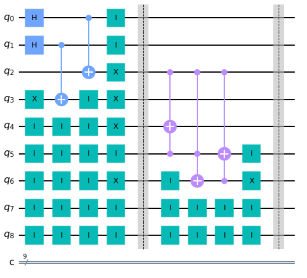
\includegraphics[scale=0.6]{background/firstAdd.png}
      \caption{First Addition: circuit}
      \label{QADD1}
\end{figure}
%%%%%%%%%%%%%%%%%%%%%%%%%%%%%%%%%%%%%%%%

The procedures carried out for the first addition, are then repeated with qubit three in place of qubit two. The code snippet in Figure \ref{QADD2} shows the resulting circuit with both additions.

%%%%%%%%%%%%%%%%%%%%%%%%%%%%%%%%%%%%%%%%
\begin{figure}[H]
      \centering
      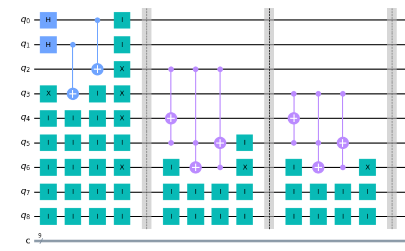
\includegraphics[scale=0.56]{background/2ndAdd.png}
      \caption{Circuit with Both Additions}
      \label{QADDFul}
\end{figure}
%%%%%%%%%%%%%%%%%%%%%%%%%%%%%%%%%%%%%%%%

%%%%%%%%%%%%%%%%%%%%%%%%%%%%%%%%%%%%%%%%
\begin{figure}[H]
      \centering
      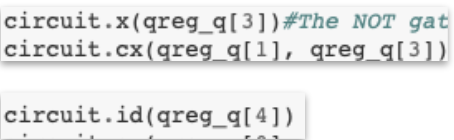
\includegraphics[scale=0.4]{background/AddCode.png}
      \caption{Second Addition: code}
      \label{QADD2}
\end{figure}
%%%%%%%%%%%%%%%%%%%%%%%%%%%%%%%%%%%%%%%%



\vspace{0.4cm}
\textbf{\underline{OR Operation}}
\vspace{0.1cm}

Following the addition operations, the condition of the Hamming distance can now be found. This is done through the application of an OR operation on the most significant bit. %To do so we need to perform an OR operation on the most significant bit. 
 Keeping with the same paper \citep{Kaye}, the illustration in Figure \ref{QORFol} is followed in order to observe the Hamming distance.

If a \emph{one} is found ,this is added to the Hamming Distance total and those with the same Hamming distance are said to be neighbours.

%%%%%%%%%%%%%%%%%%%%%%%%%%%%%%%%%%%%%%%%
\begin{figure}[H]
      \centering
      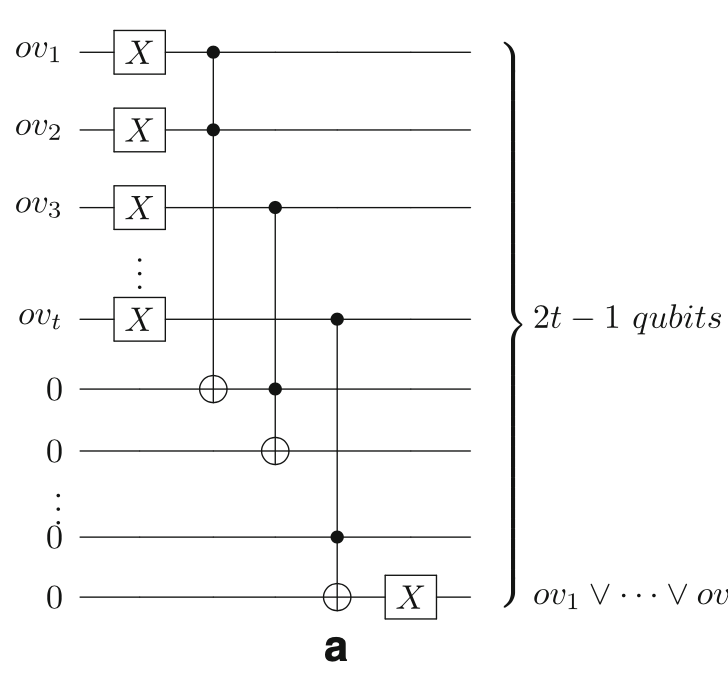
\includegraphics[scale=0.65]{background/KayeOR.png}
      \caption{OR operation: \citep{Kaye}}
      \label{QORFol}
\end{figure}
%%%%%%%%%%%%%%%%%%%%%%%%%%%%%%%%%%%%%%%%

To begin with, all inputs from the additions stored in qubit four, five and six are negated. This negation allows for a zero or a ‘1’ to be more easily detectable, with the presence of the latter depicting a neighbour.
 
To do so the following steps are applied:
\begin{enumerate}

\item Apply a toffoli gate on qubits four and five, with qubit seven as the target.
\vspace{0.3cm}

\item The second toffoli gate makes use of qubits five and six, with qubit eight acting as the target.
\vspace{0.3cm}
\end{enumerate}

Following the application of both additions and the OR operation, the resulting complete QkNN circuit is seen in Figure \ref{FKNN}.





\subsection{Quantum Support Vector Mechanism (QSVM)}\label{QSVMImp}

There are two possible directions that can be taken when implementing a Quantum Support Vector Mechanism: 

\begin{enumerate}
\item Make use of the built in Qiskit  function for QSVM.


\item Implement a QSVM circuit.
\end{enumerate}

\vspace{0.3cm}
\textbf{\underline{Function Call}}


Qiskit Aqua provides a predefined function that allows the entire QSVM kernel to be train. Figure \ref{SVMCal} depicts how this function is imported and supplied with the necessary parameters:

 - Feature map: This is a way of encoding classical data so it can be read by a quantum circuit. 
 
 - \texttt{Training$_-$input}, \texttt{Test$_-$input}: These are the data sets.
 
 
%%%%%%%%%%%%%%%%%%%%%%%%%%%%%%%%%%%%%%%%
\begin{figure}[H]
      \centering
      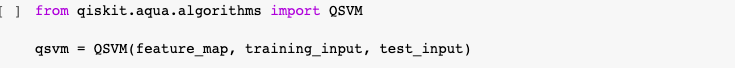
\includegraphics[scale=0.6]{background/SVMImp.png}
      \caption{QSVM: Function Call}
      \label{SVMCal}
\end{figure}
%%%%%%%%%%%%%%%%%%%%%%%%%%%%%%%%%%%%%%%%

\vspace{0.3cm}
\textbf{\underline{Circuitry}}

The implementation process for this QSVM technique can be divided into three parts: 
\begin{enumerate}
    
\item  \textbf{Data Processing:} Data processing is delivered through the use of feature maps as discussed in Section \ref{FMapIMPle}. Figure \ref{SVMFMap} shows how we can specify the feature map and the shot count for a dataset.


%%%%%%%%%%%%%%%%%%%%%%%%%%%%%%%%%%%%%%%%
\begin{figure}[H]
      \centering
      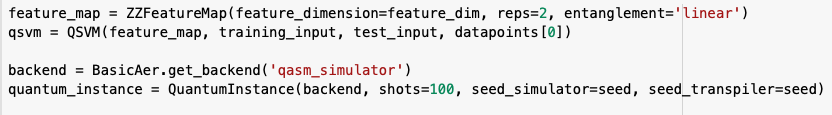
\includegraphics[scale=0.6]{background/fMapSVM.png}
      \caption{QSVM: Feature Mapping}
      \label{SVMFMap}
\end{figure}
%%%%%%%%%%%%%%%%%%%%%%%%%%%%%%%%%%%%%%%%



\item \textbf{Generation of the unitary operator:} Figure \ref{SVMCir} shows the generation of the unitary operator, with a circuit composed of unitary gates and controlled not gates. The U gate is similar to the Ry gates, as it used for encoding classical data within the Bloch sphere. The U gates encodes this data by mapping the data around the $Z-axis$. \emph{P.A McRae, M. Hilkea} \citep{mcrae2020} go more in depth into this implementation design, but with their direction the QSVM circuit can be implemented in Figure \ref{SVMCir} .

%%%%%%%%%%%%%%%%%%%%%%%%%%%%%%%%%%%%%%%%
\begin{figure}[H]
      \centering
      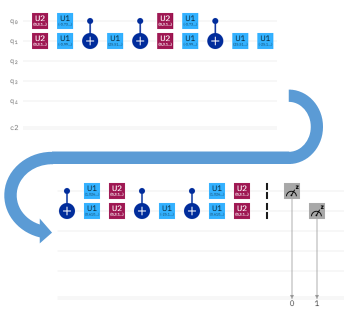
\includegraphics[scale=0.8]{background/SVMCir.png}
      \caption{QSVM: Circuit \cite{mcrae2020}}
      \label{SVMCir}
\end{figure}
%%%%%%%%%%%%%%%%%%%%%%%%%%%%%%%%%%%%%%%%

\item \textbf{Generation of the kernel matrix K:} After the classical data is now encoded into  quantum data it is supplied to the QSVM kernel. The kernel matrix in this implementation is the same as the classical SVM kernel but with quantum encoded data points. Using Python we can  make use of the function call shown in Figure \ref{SVMKer} to generate the kernel for our dataset.

%%%%%%%%%%%%%%%%%%%%%%%%%%%%%%%%%%%%%%%%
\begin{figure}[H]
      \centering
      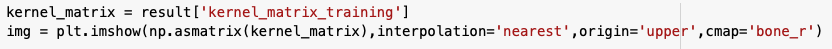
\includegraphics[scale=0.5]{background/Kernal.png}
      \caption{QSVM: Kernel Code} %\cite{mcrae2020}}
      \label{SVMKer}
\end{figure}
%%%%%%%%%%%%%%%%%%%%%%%%%%%%%%%%%%%%%%%%
\end{enumerate}



%These steps are then followed by a readout preformed through measurement.
%With their direction we can implement the following QSVM circuit. 

\subsection{Grover's Search Algorithm}

Similar to 2.1.2, two directions can be taken when implementing Grover's Search algorithm:
\begin{enumerate}

\item Make use of the built in Qiskit “black box” function.

\item Implement a Grover's Search circuit.
\end{enumerate}

\vspace{0.3cm}
\textbf{\underline{Function Call}}


Similar to QSVM, Qiskit Aqua provides a predefined function to perform Grover's Search algorithm. Using Qiskit we first call the import function, then the oracle. The oracle acts as a black box reference to the Grover's Search circuit, which will only require the testing data as inputs. 

%Grover's function call only requires the test data parameter. In this case for the 3SAT satisfiability data. 

%%%%%%%%%%%%%%%%%%%%%%%%%%%%%%%%%%%%%%%%
\begin{figure}[H]
      \centering
      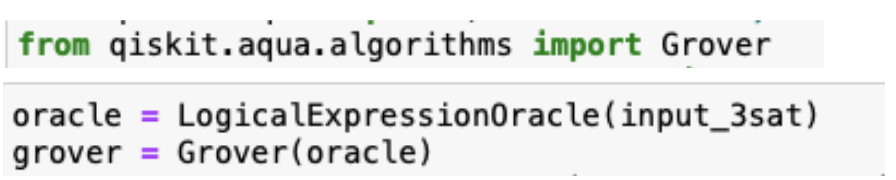
\includegraphics[scale=0.6]{background/GroverImp.png}
      \caption{Grover's Search Algorithm: Function Call}
      \label{GrvImp}
\end{figure}
%%%%%%%%%%%%%%%%%%%%%%%%%%%%%%%%%%%%%%%%


\vspace{0.3cm}
\textbf{\underline{Circuitry}}

With Grover's Search algorithm, the circuit changes depending on the number of qubits and iterations needed. This implementation will be focusing on a four qubit circuit with one circuit iteration. 
Following the same guide as the QSVM circuit, we will implement another design from %\emph{P.A McRae, M. Hilkea} 
\citep{mcrae2020}, where different rotations of Grover's Search with multiple iterations are more extensively covered.  

%%%%%%%%%%%%%%%%%%%%%%%%%%%%%%%%%%%%%%%%
\begin{figure}[H]
      \centering
      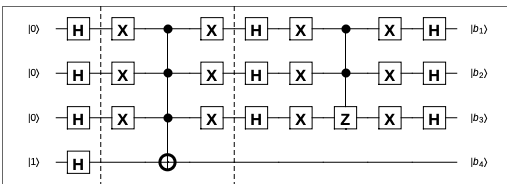
\includegraphics[scale=0.8]{background/GroverCir.png}
      \caption{Grovers Search: Circuit \cite{mcrae2020}}
      \label{GrvCir}
\end{figure}
%%%%%%%%%%%%%%%%%%%%%%%%%%%%%%%%%%%%%%%%


Grover's Circuit is composed of three stages:

\begin{enumerate}
    \item \textbf{Initialisation:} During the initialisation stage, all qubits are placed into superposition using the H gate.
    
    This ensures all the qubits have the same probability amplitude or have the same expected value.
   
    
    \item \textbf{The Oracle:} The oracle is the black box function that the Qiskit function call initiates. 
    
    The oracle function marks the state $x'$ that satisfies the condition $f(x')$ = 1 by performing a phase flip. All other states are left unaltered. The operation has the effect of inverting the state’s amplitude and it runs in constant time.
    
    This is implemented through marking the target element by negating its sign or applying a gate operation flip.
    
    \item \textbf{Amplitude Amplification:} Amplitude Amplification amplifies the amplitudes of the desired element. It is applied to eliminate one-sided error from the inputs  retrieved from the oracle.

Applying these steps to a single qubit Grover's circuit would deliver Figure \ref{GrovCirImple1QBit}
%%%%%%%%%%%%%%%%%%%%%%%%%%%%%%%%%%%%%%%%
\begin{figure}[H]
      \centering
      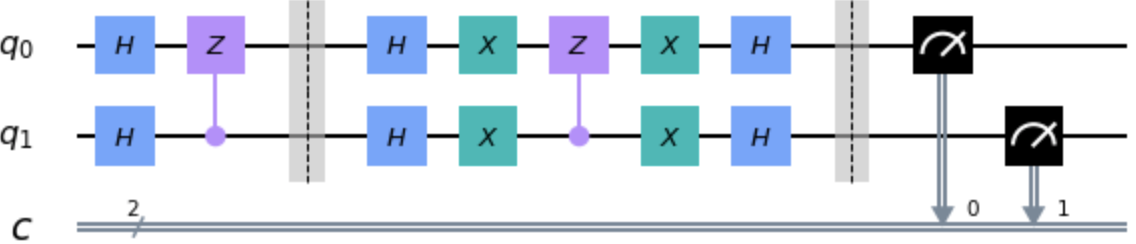
\includegraphics[scale=0.5]{background/Grovers1Bit.png}
      \caption{Grovers Search: 1 Qubit Implemented Circuit}
      \label{GrovCirImple1QBit}
\end{figure}
%%%%%%%%%%%%%%%%%%%%%%%%%%%%%%%%%%%%%%%%

\end{enumerate}

These steps, for a full four qubit circuit would result in the circuit %of this implemented circuit is 
 illustrated in Figure \ref{GrovCirImple}.
%%%%%%%%%%%%%%%%%%%%%%%%%%%%%%%%%%%%%%%%
\begin{figure}[H]
      \centering
      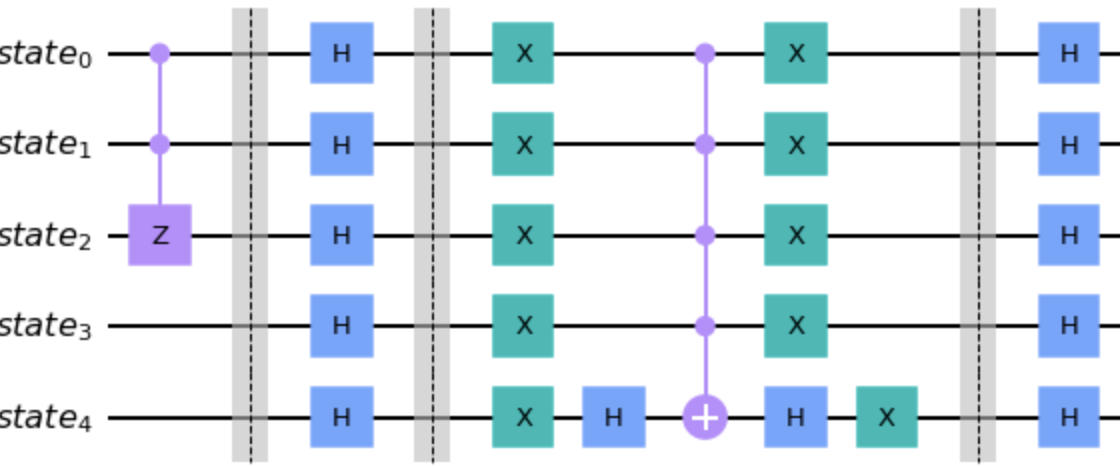
\includegraphics[scale=0.5]{background/Grover_non_or.png}
      \caption{Grovers Search: Implemented Circuit}
      \label{GrovCirImple}
\end{figure}
%%%%%%%%%%%%%%%%%%%%%%%%%%%%%%%%%%%%%%%%

Since a four qubit Toffoli or Controlled Controlled Not (CCNOT) gate is not supported by Qiskit, it can be implemented % the four qubit Toffoli or Controlled Controlled Not (CCx) gate can be implemented
using the Qiskit multi-qubit controlled not gate (MCMT), where the control qubits are specified first then the target qubit.:
 
 \texttt{MCMT.ccx(q[2], q[0], q[1], q[3], ctl1=None, ctl2=None, tgt=None)}.
 
Another option is to repeat the steps for the single qubit implementation above but repeated for each qubit operation as seen in Figure \ref{GrovCirImple4Bit}.

%%%%%%%%%%%%%%%%%%%%%%%%%%%%%%%%%%%%%%%%
\begin{figure}[H]
      \centering
      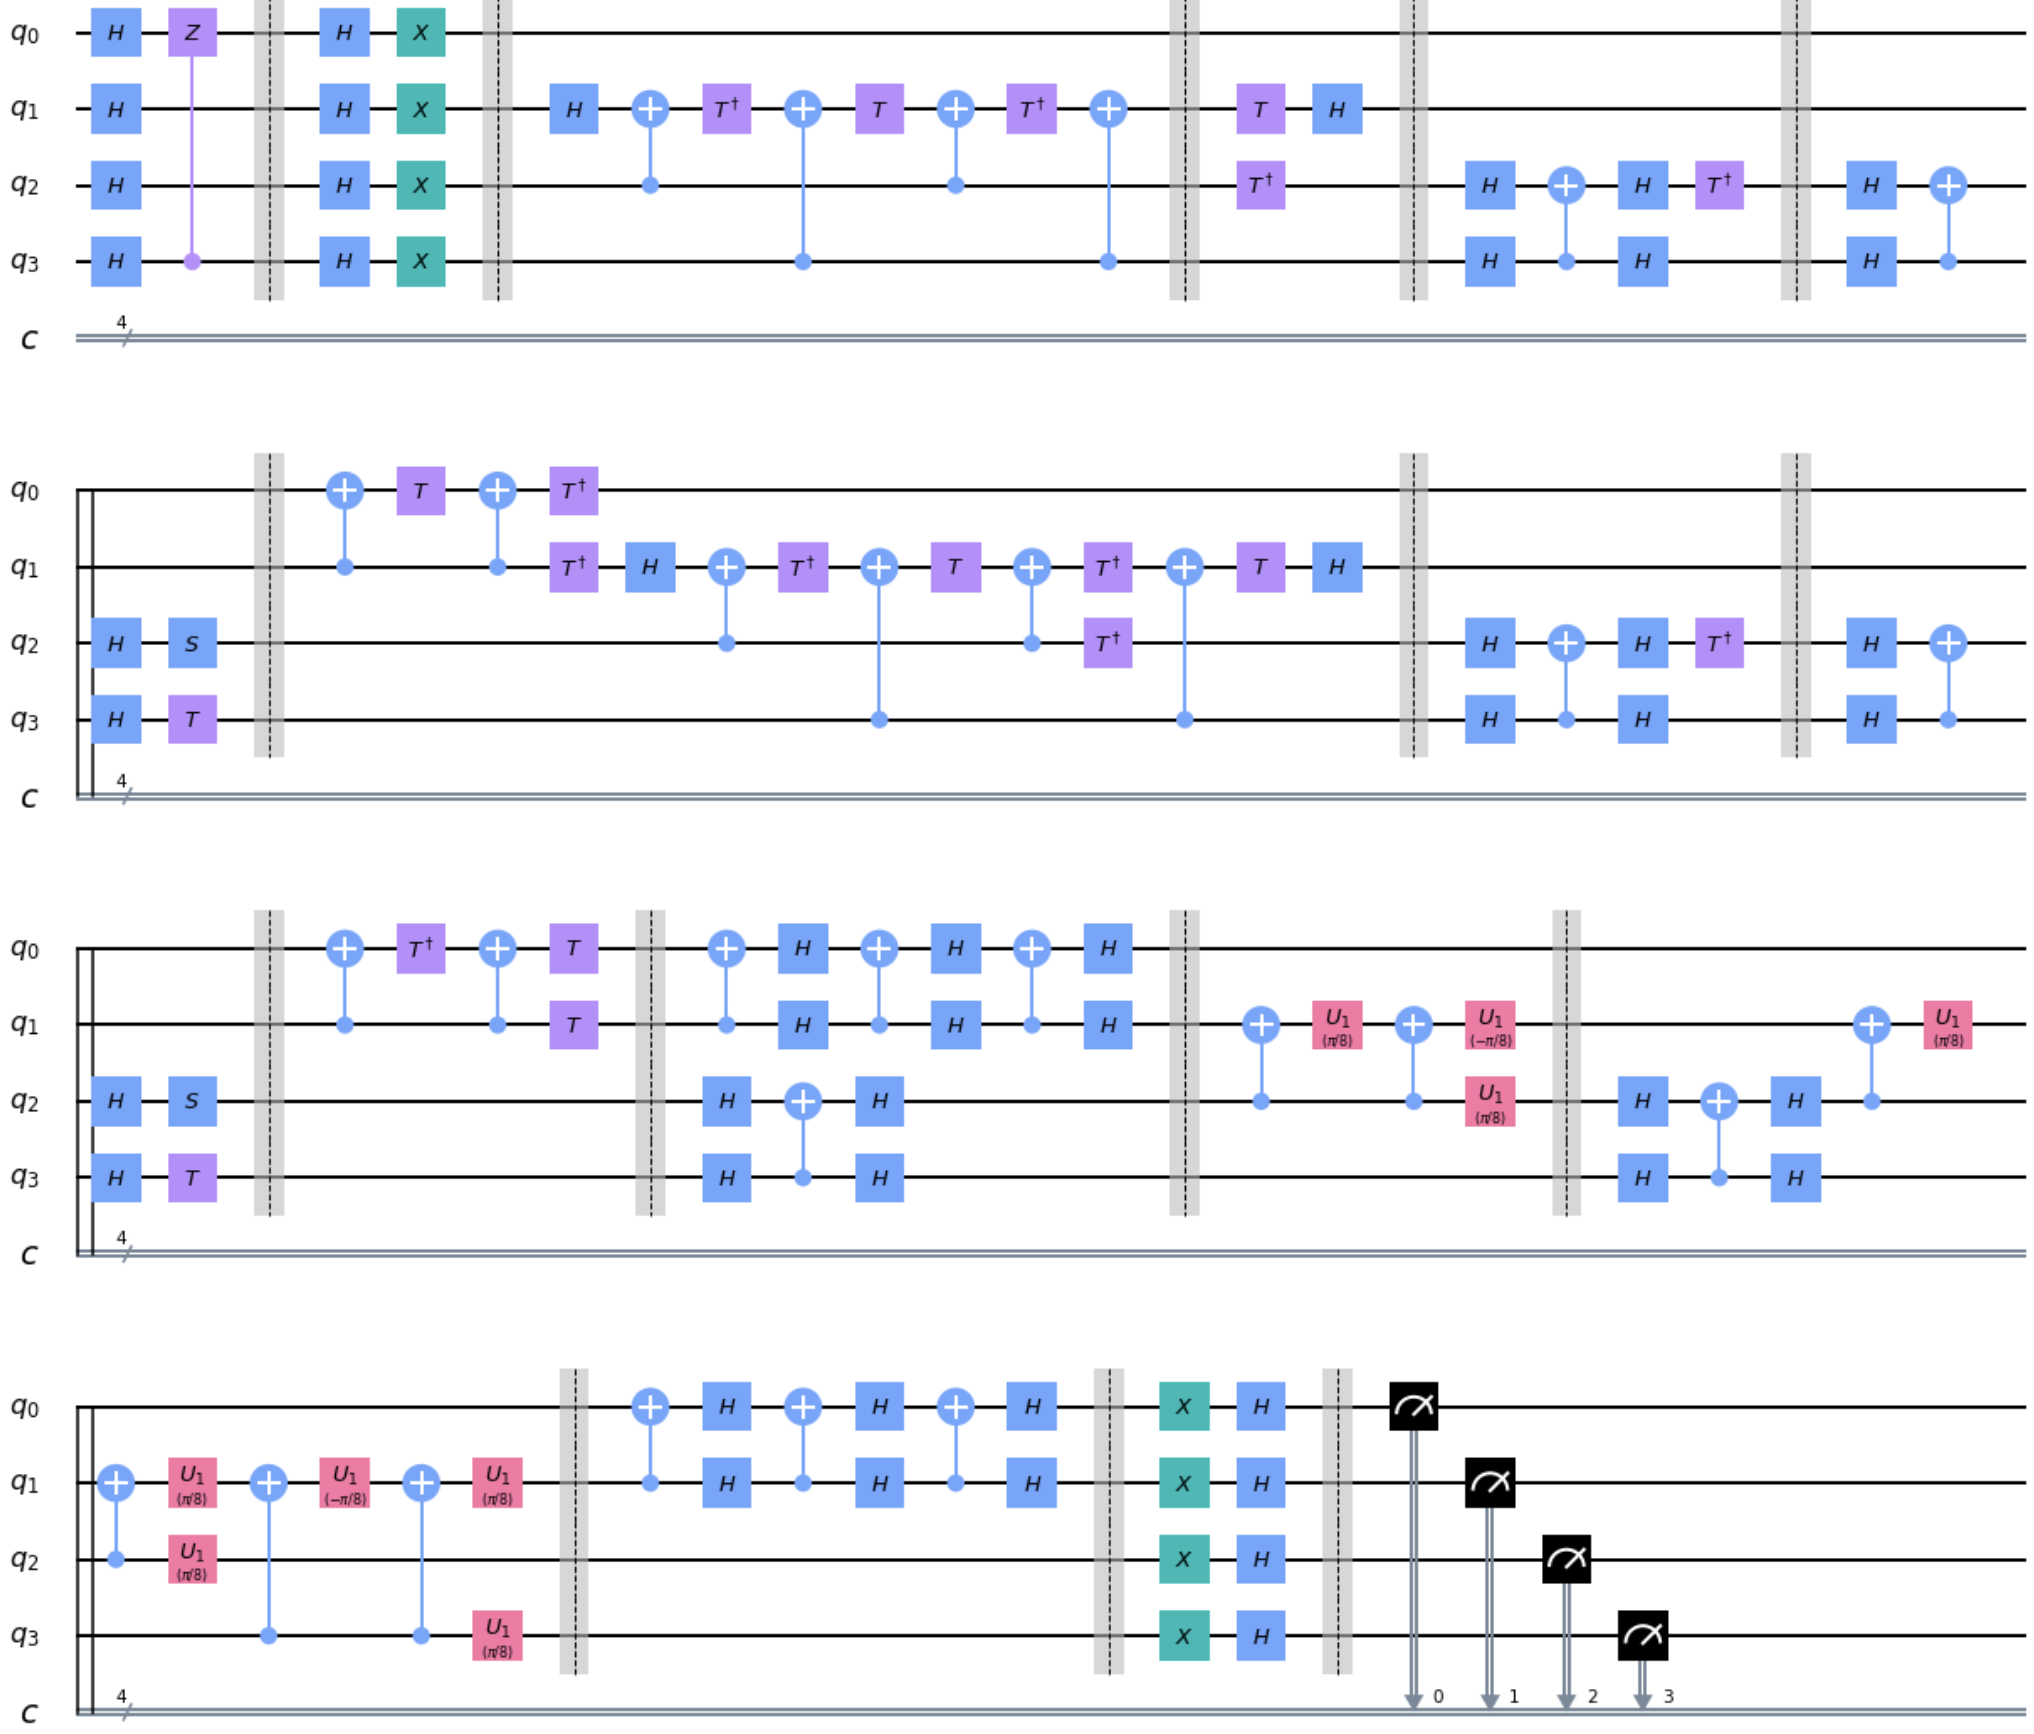
\includegraphics[scale=0.4]{background/Grovers4Bits.png}
      \caption{Grovers Search: Implemented 4 Bit Circuit}
      \label{GrovCirImple4Bit}
\end{figure}
%%%%%%%%%%%%%%%%%%%%%%%%%%%%%%%%%%%%%%%%

\section{Measurements and Subroutines}
To enable the circuit components in the quantum tool to be modular, quantum subroutines are used. This modular circuit can then be evaluated using a quantum machine. In order to evaluate the circuit output, a measurement must be taken. 

\subsection{Subroutines}
Each algorithm and data encoding operation currently resides and are compiled in linear order in their code blocks e.g in a Jupyter notebook. These code blocks can be encapsulated as subroutines. Subroutines not only provide a visual representation of the circuit components but they also enable these components to be modular.
Taking the feature mapping operation as an example, to be able to manipulate it as a subroutine one must:

\begin{enumerate}

\item Specify the number of qubits needed, in this case four.

\item Define the circuit by providing a name of the subroutine.

%%%%%%%%%%%%%%%%%%%%%%%%%%%%%%%%%%%%%%%%
\begin{figure}[H]
      \centering
      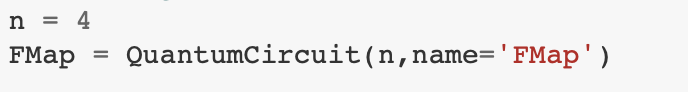
\includegraphics[scale=0.8]{background/SubR1.png}
      \caption{Feature Map Encoding Subroutine: Steps 1 and 2}
      \label{SUR1}
\end{figure}
%%%%%%%%%%%%%%%%%%%%%%%%%%%%%%%%%%%%%%%%


\item Carry out the feature mapping operation.

\item Set the feature map circuit to the subroutine as shown in Figure \ref{SUR2}.

\item Call the \texttt{to$_-$gate()} function in Figure \ref{SUR2}, to enable the subroutine to be called and manipulated at any point in the circuit. 

\end{enumerate}

%%%%%%%%%%%%%%%%%%%%%%%%%%%%%%%%%%%%%%%%
\begin{figure}[H]
      \centering
      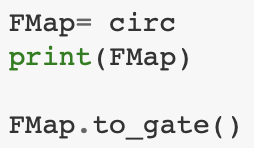
\includegraphics[scale=0.8]{background/SubR2.png}
      \caption{Encoding Feature Map Subroutine: Steps 4 and 5}
      \label{SUR2}
\end{figure}
%%%%%%%%%%%%%%%%%%%%%%%%%%%%%%%%%%%%%%%%

%%%%%%%%%%%%%%%%%%%%%%%%%%%%%%%%%%%%%%%%
\begin{figure}[H]
      \centering
      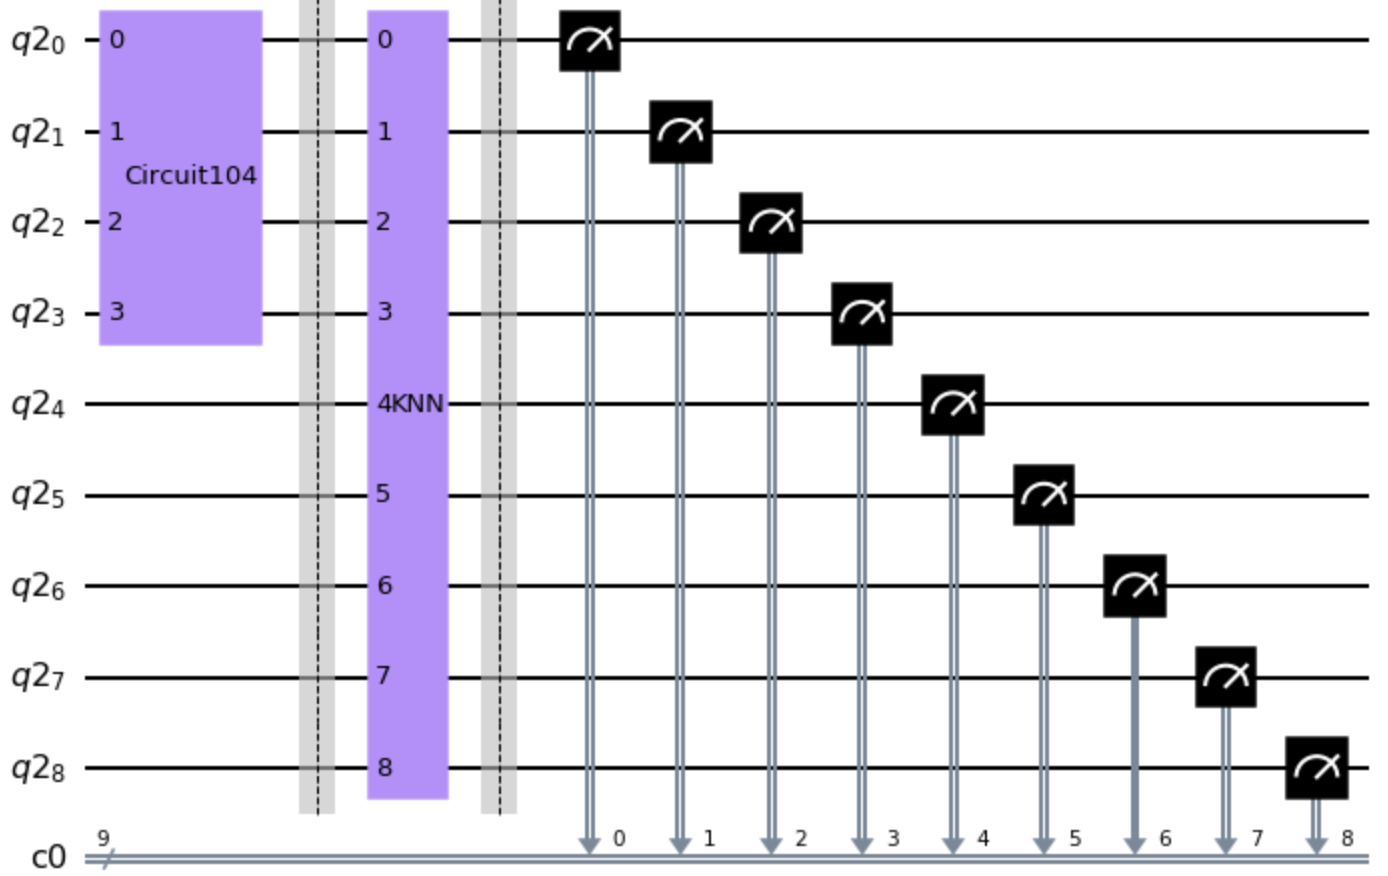
\includegraphics[scale=0.5]{background/FullSubR.png}
      \caption{Subroutines: QKNN and Feature Mapping Circuit }
      \label{FullSR}
\end{figure}
%%%%%%%%%%%%%%%%%%%%%%%%%%%%%%%%%%%%%%%%

The same process can also be applied to the QkNN circuit, this data encoding and quantum algorithm combination results in the circuit shown in Figure \ref{FullSR}.





\subsection{Measurements}

At the end of Figure \ref{FullSR}, there are an array of black time dials, these are measurements. In order to run the complete circuit the measurements of each qubit must be taken. This measurement causes the superposition of the qubit to collapse and forces the qubits to reveal their state.

With the use of the Qiskit's measure function shown in Figure \ref{Mes}, the full circuit can be measured by supplying all used qubits. Individual qubits can also be tested during the circuit construction in order to check for a desired outcome.
 

%%%%%%%%%%%%%%%%%%%%%%%%%%%%%%%%%%%%%%%%
\begin{figure}[H]
      \centering
      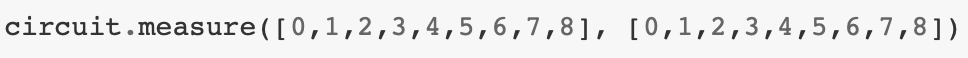
\includegraphics[scale=0.8]{background/Measure.png}
      \caption{Taking Circuit Measurements  }
      \label{Mes}
\end{figure}
%%%%%%%%%%%%%%%%%%%%%%%%%%%%%%%%%%%%%%%%



\section{Quantum Execution}
The completed circuits can now be run on a quantum computer however, there are a few preliminary steps that must be addressed.
To begin with, an IBM Q Experience account is needed, so it must be created. % to first create an IBM Q Experience account,
Following the creation of the IBM account, the provided IBM access code  needs to be noted. % of our IBM access code.
Finally with the IBM account, the access code can be loaded into the Qiskit code, as seen in Figure \ref{IBMSet}. 

%%%%%%%%%%%%%%%%%%%%%%%%%%%%%%%%%%%%%%%%
\begin{figure}[H]
      \centering
      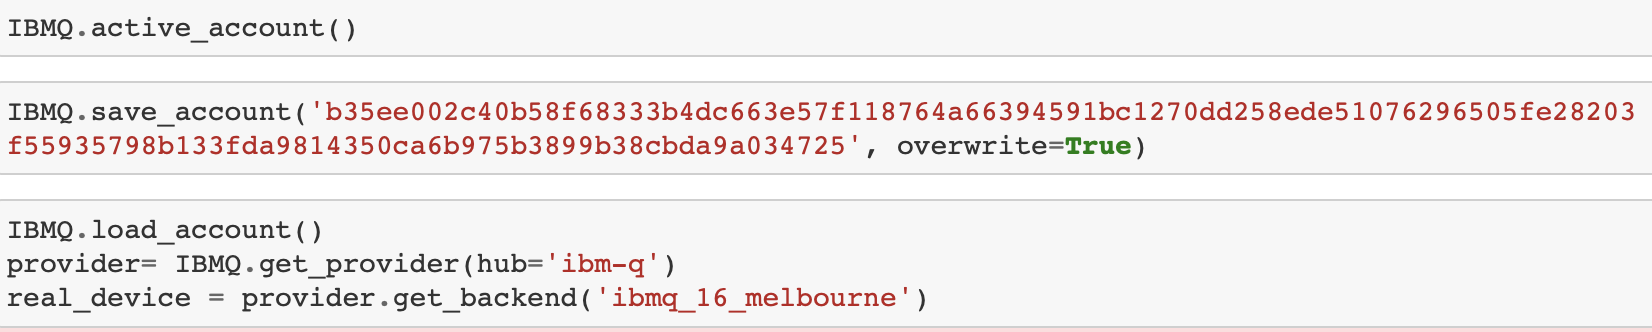
\includegraphics[scale=0.5]{background/IBMStart.png}
      \caption{IBM Quantum Experience Setup }
      \label{IBMSet}
\end{figure}
%%%%%%%%%%%%%%%%%%%%%%%%%%%%%%%%%%%%%%%%

The Qiskit back-end that will run the circuit needs to specified. It is necessary to choose an appropriate back-end with the equivalent quantum volume availability. As seen in Figure \ref{QMachineAvail},  the maximum size of the implemented quantum circuit is the size of the quantum machine that must be chosen. 
With the largest implemented circuit (the QkNN circuit) using nine qubits, the Melbourne device is the only option as it allows for a 15 qubit volume and it is currently online. 


%%%%%%%%%%%%%%%%%%%%%%%%%%%%%%%%%%%%%%%%
\begin{figure}[H]
      \centering
      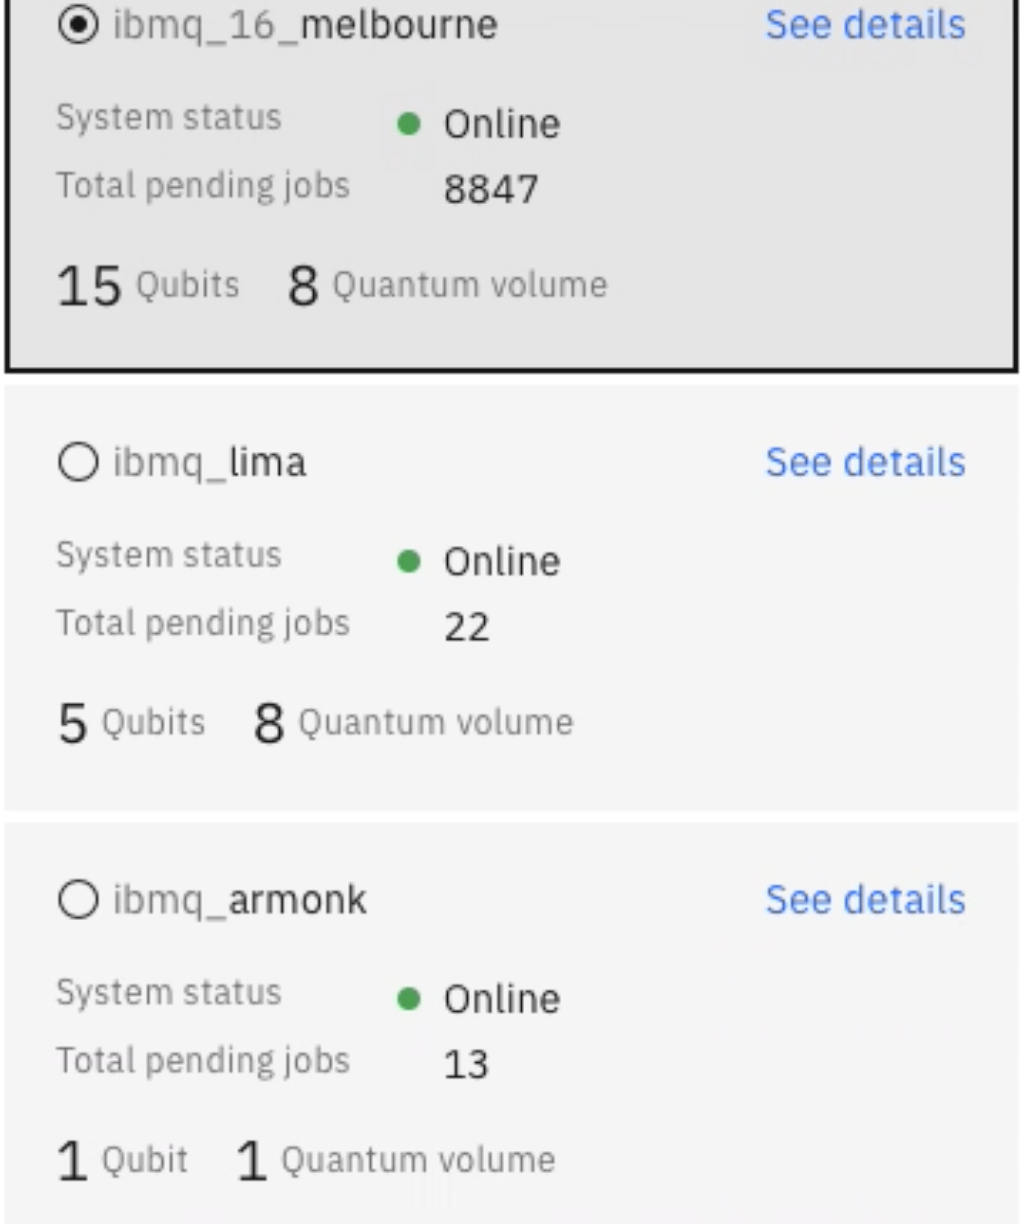
\includegraphics[scale=0.4]{background/QMachineOptions.png}
      \caption{ Quantum Machine Available }
      \label{QMachineAvail}
\end{figure}
%%%%%%%%%%%%%%%%%%%%%%%%%%%%%%%%%%%%%%%%


\subsection{Quantum Simulation}

Before, the circuit can be executed on a quantum machine, it first needs to simulated. This simulation ensures that one is not presented with an \emph{‘error running jobs’} alert, and thus the circuit is executable. 

As shown in Figure \ref{QSim}, the simulator is initially called, then the simulation can be executed by providing the number of shots desired. As qubits in superposition are random, sometimes 0, sometimes 1, or a probability of both, shots allows for repeat measurements. This re-measurement  determines the likelihood that a qubit is in a particular state. Following the simulation, the circuit results are then visualised.

%%%%%%%%%%%%%%%%%%%%%%%%%%%%%%%%%%%%%%%%
\begin{figure}[H]
      \centering
      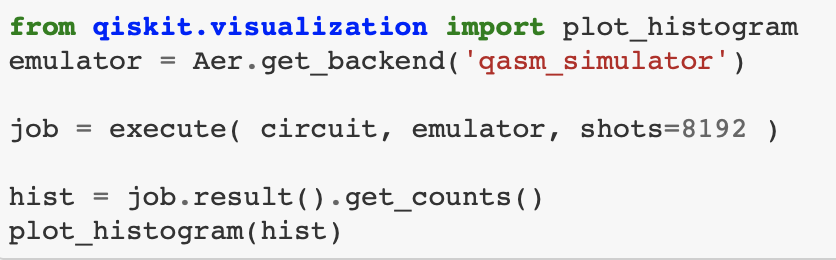
\includegraphics[scale=0.4]{background/QExSim.png}
      \caption{Quantum Simulator: setting up the simulator for circuit execution and plotting the results}
      \label{QSim}
\end{figure}
%%%%%%%%%%%%%%%%%%%%%%%%%%%%%%%%%%%%%%%%
 


\subsection{Quantum Run}

Running a circuit on a quantum machine follows the same procedure as the quantum simulation. As seen in Figure \ref{QRun}, the only difference is the use of the quantum device (\texttt{backend = real\_device}) that was initiated in Figure \ref{IBMSet}; the shot counts number and the return parameter \texttt{run$_-$id} are also specified. The \texttt{run$_-$id} parameter enables one to keep track of the current execution state, using this parameter the quantum run outputs can then plotted in order to visualise the result.

%%%%%%%%%%%%%%%%%%%%%%%%%%%%%%%%%%%%%%%%
\begin{figure}[H]
      \centering
      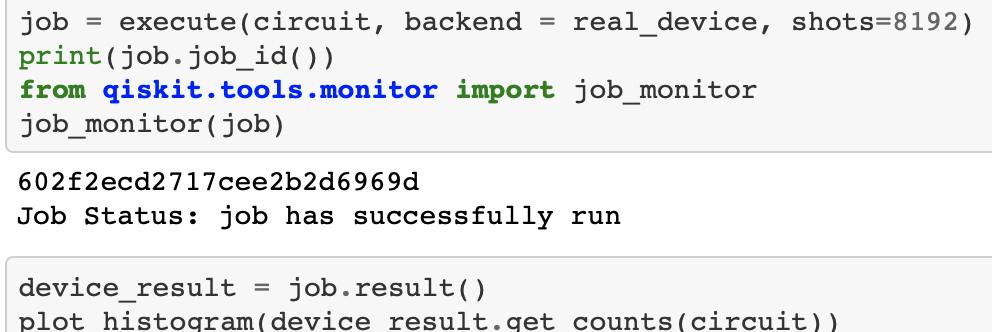
\includegraphics[scale=0.7]{background/QRun.png}
      \caption{Quantum Machine Execution: running the circuit on a quantum computer }
      \label{QRun}
\end{figure}
%%%%%%%%%%%%%%%%%%%%%%%%%%%%%%%%%%%%%%%%

\section{Classical Simulation of Quantum Circuits: JKU Implementation }

%\subsection{JKU Implementation}

%With our newly obtained quantum results, using 
The JKU simulator enables quantum circuits to executed on a simulation of a classical computer. Figure \ref{JK1} depicts how to import and create an instance of the JKU simulator.

%%%%%%%%%%%%%%%%%%%%%%%%%%%%%%%%%%%%%%%%
\begin{figure}[H]
      \centering
      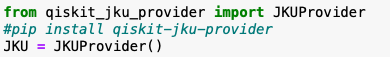
\includegraphics[scale=0.7]{background/JK1.png}
      \caption{JKU Simulator: Import and Setup code  }
      \label{JK1}
\end{figure}
%%%%%%%%%%%%%%%%%%%%%%%%%%%%%%%%%%%%%%%%

Using the code snippet in Figure \ref{JK2}, the JKU backend can be called from the JKU provider. This backend allows for the circuit to be simulated and then retrieved, from which the circuit results can be displayed.% the results.
%%%%%%%%%%%%%%%%%%%%%%%%%%%%%%%%%%%%%%%%
\begin{figure}[H]
      \centering
      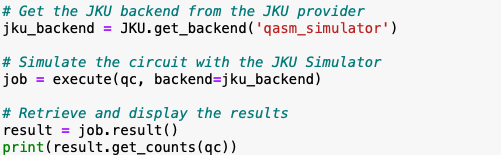
\includegraphics[scale=0.6]{background/JK2.png}
      \caption{JKU Simulator: code to run JKU, execute the simulator and retrieve results}
      \label{JK2}
\end{figure}
%%%%%%%%%%%%%%%%%%%%%%%%%%%%%%%%%%%%%%%%
\vspace{0.4cm}



\subsection{Error Handling}

With Qiskit and classical simulators being relatively new, there are some errors that one will encounter. The open source community for JKU and Qiskit are active and available to help.


\vspace{0.4cm}
\textbf{\underline{Coupling Map Error}}

One such error is the coupling map error, which is presented as a trace-back error when the JKU instance is initially called. 

%%%%%%%%%%%%%%%%%%%%%%%%%%%%%%%%%%%%%%%%
\begin{figure}[H]
      \centering
      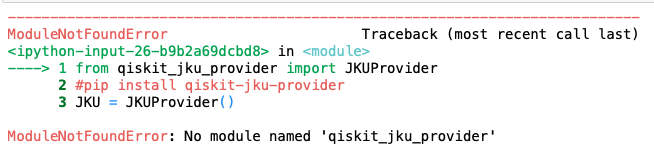
\includegraphics[scale=0.5]{background/ERRH.png}
      \caption{Expected error code output for Coupling Map error }
      \label{ERRC}
\end{figure}
%%%%%%%%%%%%%%%%%%%%%%%%%%%%%%%%%%%%%%%%
Figure \ref{CMapFix} illustrates the solution for this error, which requires one to locate the \texttt{quasm$_-$simulator$_-$jk.py} file from the location in the system where the JKU import was saved. When this file location is obtained one can then manoeuvre to the QasmSimulator class, there %we will come across 
the \texttt{DEFAULT$_-$CONFIGURATION} section can be found. Finally, in that \texttt{DEFAULT$_-$CONFIGURATION} section the line, \emph{coupling$_-$map: None,} needs to be included.



%%%%%%%%%%%%%%%%%%%%%%%%%%%%%%%%%%%%%%%%
\begin{figure}[H]
      \centering
      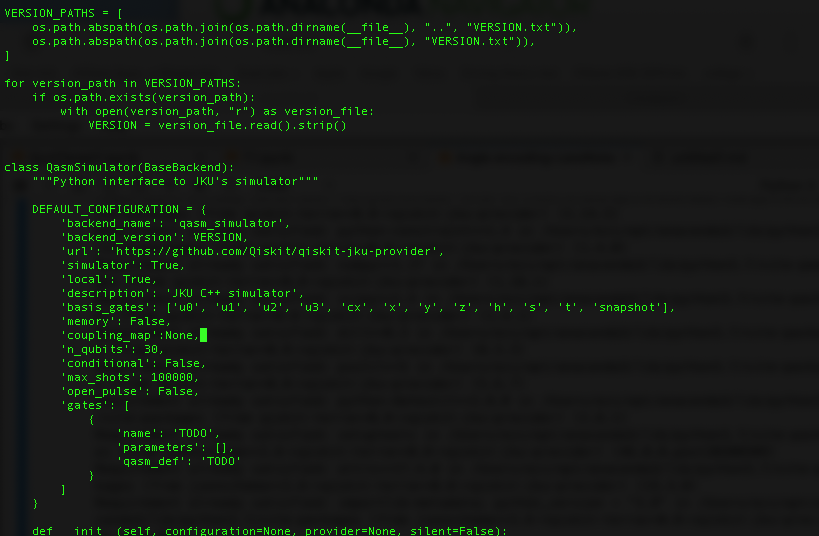
\includegraphics[scale=0.6]{background/CouplinMapFix.png}
      \caption{ Coupling Map error: Error Code Fix }
      \label{CMapFix}
\end{figure}
%%%%%%%%%%%%%%%%%%%%%%%%%%%%%%%%%%%%%%%%

\vspace{0.4cm}
\textbf{\underline{Identity Gate Error}}

The JKU simulator is built upon Qiskit's open source simulators. When Qiskit updates its simulators, these updates need to manually propagated to the JKU simulator. One such update is Qiskit backend simulator no longer automatically removing identity (ID) gates; \emph{``IBMQ backends, for example, have traditionally implemented id gates as an implicit delay, though this behaviour will be removed in the future.''} \citep{PersonalQiskit} 

One possible fix would see the removal of the ID gates from ones circuit, if that does not fix the error -- such was the case in this dissertation -- one has to wait or can contribute to this update propagation within the JKU open source library.

%usually ID gates are ignored or removed as no operation is applied to that gate for one unit of time.